% inspired from http://tex.stackexchange.com/questions/26370/how-to-draw-stack-diagram-with-tikz 
% and http://tex.stackexchange.com/questions/52761/tikz-diagram-with-stacks-and-box
\documentclass{article}

\usepackage[utf8]{inputenc}
\usepackage[T1]{fontenc}
\usepackage{tikz}
\usetikzlibrary{shapes, positioning, arrows, calc}

\begin{document}

% pile : exemple

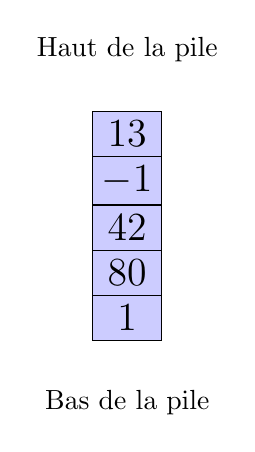
\begin{tikzpicture}[stack/.style = {fill = blue!20, font = \sffamily\Large\bfseries, rectangle split, rectangle split parts = 5, draw, anchor = center}]
   \node [stack] (stack)  {$13$\nodepart{two}$-1$
   \nodepart{three}$42$\nodepart{four}$80$\nodepart{five}$1$};
   \node [above = 0.5cm of stack, align = left] {Haut de la pile};
   \node [below = 0.5cm of stack, align = left] {Bas de la pile};
\end{tikzpicture}

% pile : exemple ajout

\vspace{3cm}
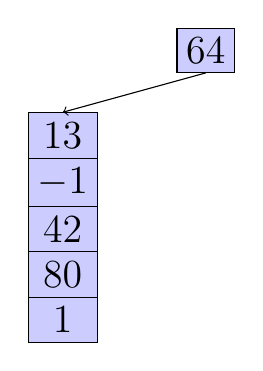
\begin{tikzpicture}[stack/.style = {fill = blue!20, font = \sffamily\Large\bfseries, rectangle split, rectangle split parts = 5, draw, anchor = center}, new/.style = {fill = blue!20, font = \sffamily\Large\bfseries, rectangle, draw, anchor = center}]
   \node [stack] (stack)  {$13$\nodepart{two}$-1$
   \nodepart{three}$42$\nodepart{four}$80$\nodepart{five}$1$};

   \node [new, above right = 0.5cm and 1cm of stack] (n) {$64$};
   \draw [->] (n.south) -- (stack.north);
\end{tikzpicture}

% pile : exemple suppression

\vspace{3cm}
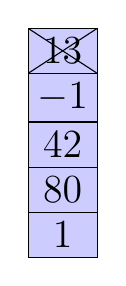
\begin{tikzpicture}[stack/.style = {fill = blue!20, font = \sffamily\Large\bfseries, rectangle split, rectangle split parts = 5, draw, anchor = center}]
   \node [stack] (stack)  {$13$\nodepart{two}$-1$
   \nodepart{three}$42$\nodepart{four}$80$\nodepart{five}$1$};

   \draw (0.43,1.45) -- (-0.43,0.89);
   \draw (0.43,0.89) -- (-0.43,1.45);
\end{tikzpicture}

\end{document}
